\documentclass[11pt]{article}

\usepackage{float}
\usepackage{amsmath}
\usepackage{amssymb}
\usepackage{geometry}
\usepackage{graphicx}
\usepackage{tikz}
\usepackage{epstopdf}
\usepackage{caption}
\usepackage{subcaption}
\usepackage{hyperref}
\usepackage[author={Harish}]{pdfcomment}

\geometry{letterpaper,tmargin=1in,bmargin=1in,lmargin=1in,rmargin=1in}
\hypersetup{colorlinks,linkcolor=black,citecolor=violet,urlcolor=magenta}

\begin{document}

\begin{center}

\large
\topskip0pt
\vspace*{\fill}
Design and Development of\\
\textbf{Remote Vibration Monitoring Sensor}

\vspace{2cm}

Design 2 - Final Report \\
Florida Polytechnic University \\
Spring 2017\\

\vspace{2cm}
Submitted by:\\
Smart Vibes\\
Ezequiel Juarez Garcia\\
Marc-Edwin Rigaud\\
Jordan Faison\\
Joshua Watkins
\vspace*{\fill}

\end{center}

\newpage

\tableofcontents

\newpage

%% Section
\section{Introduction}

As a Design 2 class project, Smart Vibes set out to create a remote vibration monitoring solution for the company Smart Structures. Smart Structures is a company that uses embedded data collectors cast into concrete to wirelessly transmit vibration monitoring information. They were looking for a sensor that could monitor vibrations at a construction site in a portable fashion. The sensor would have to monitor the magnitude and frequency composition of vibrations created by machinery. Based off of regulations and standards, the sensor would trigger an alarm when vibrations exceeded certain magnitude and frequency thresholds. The thresholds would be lower than the actual values that it would take to compromise the integrity of surrounding buildings. The alarm would notify workers on site and log the event on the sensor and on a remote server. A daily log of events and alarms would be accessible on a cloud platform for the company to review at their leisure.

The project began with a phone call to Smart Structures to learn more about the system requirements of the sensor. In the preliminary design stage, we discussed how the sensor would satisfy the system requirements and what components we were going to use. Following that, we created the system level requirements for the sensor, conceived the structural and software design, and began researching for the optimal components for the sensor. After creating the bill of materials, we waited a couple of weeks for our parts to arrive.

Now, we have a prototype ready to demonstrate. We've been building and iterating on this prototype for the past two months. Throughout the prototyping process, we faced and overcame various challenges and hurdles. Getting the sensor to connect to the Microsoft Azure cloud platform was one of the greatest achievements in the project but also one of the most challenging aspects of it. The reason being that the free credits that we were given at the beginning of the trial disappeared in a matter days without us knowing why.

However, even with the cloud platform problem and other limitations that have been present along the way, our vibration sensor has the majority of the functionalities that we desired for it to have. It is open to improvements that we or Smart Structures would like to add in the future.

%% Section
\section{Customer Needs, Objectives, and Team Interpretation}

This section states the design problem and customer needs for the sensor. Using the customer needs, we created the engineering requirements for the sensor. The requirements dictated the desired functionalities of the sensor. The way our team chose to tackle those requirements, such as the decision of what components to use, shape of the design,  and final prototype of the sensor.

\subsection{Customer Needs}

Smart Structures was looking for three main qualities in the vibration sensor. The first quality was that it needed be portable. Their current products were fixed solutions, like their concrete embedded data collectors. Which is why they wanted a sensor that could be moved from site to site. The second quality/functionality they asked for, was a sensor capable of lasting close to four weeks on a single charge. The reason being that the sensor would not always be next to a power outlet to connect into. The final quality was a sensor that could collect data and upload a daily log to a cloud database. This also included sending alerts when vibrations exceeded a certain threshold, so that the responsible personnel would be aware of dangerous vibration levels. A remote solution would eliminate the need to go to the site and connect directly to the sensor to retrieve the collected data.
	
\subsection{Design Objectives}

From what we gathered from the customer needs that Smart Structures presented to us, we were able to come up with a short list of engineering requirements. The sensor would have to meet these requirements in order to function as desired.

The engineering requirements that we came up with were the following.
\begin{itemize}
\item The sensor would by made portable by using a microcontroller instead of a microcomputer or embedded system. The sensor also needed to be small.
\item A long-battery life would be made possible by using low-power electronics with power-saving capabilities.
\item The sensor would be able to transmit to the cloud by using a microcontroller with a WiFi chip on board.
\end{itemize}

\subsection{Team Interpretation}

From our customer needs, we were constrained to a few factors, the major one being data transmission given that power was a limitation. Our first thought was to find a power efficient microcontroller. The microcontroller needed transmit data wirelessly and take in large amounts of sensor data per second. We then needed to establish how we were going to get the vibration data. This led us to two different approaches to data collection: an accelerometer which outputs a digital signal and a geophone which outputs an analog signal. The integration of both of these sensors would allow for redundancy and double-checking of readings. A database was necessary to host the sensor data as well as alerts of events that occurred throughout the day.

From the interpretation of the customer needs, we were able to come up with a list of specifications for the vibrations sensor. The following are the specifications:

\begin{itemize}
\item Accelerometer and geophone would be used to collect vibrations
\item The minimum frequency that the sensor would monitor was 8 Hz
\item Data would be locally stored on an SD card
\item Alarms would be computed on the cloud and trigger an alarm on the sensor
\item Remote access and monitoring would be provided by an existing cloud platform
\item Four-week power time would be complemented by a solar panel
\end{itemize}

%% Section
\section{Concept Generation and Analysis of Alternatives}

During the concept generation stage of the project, we were able to generate the sensor specifications listed in the previous section. This section highlights the thought process behind the design of the sensor. Although we had a hard time in the beginning with the sensor design, as the semester progressed, we were able to flesh out the parts we weren't so sure about.

\subsection{Concept Generation}
The first concepts of our design were took some time to generate because of the lack of information to go on from Smart Structures. We didn't exactly know how it would all fit together until we revisited the customer needs and came up with solid system specifications and requirements. After doing that, we were able to sit and plan the physical layout of the sensor. 

At the center of the project would be a microcontroller which would take in the inputs from the sensors and upload the data to the cloud. The original briefcase model for the sensor enclosure was scrapped when we realized how large the size footprint was and how it would undermine the portability of the sensor.

%We also did not know the power consumption that was required by different processors, raspberry pi for example, had all the capabilities you could imagine, however the it consumes massive amounts of power for discrete electronics, that essentially had to be self sustaining. A lot of research went into initial concepts and throughout the entire project, many of which could still potentially be optimized.    

\subsection{Analysis of Alternatives}

In doing our project, there were more ways than one to get the desired results. We opted for parts that we knew would work together and were easily assessable.  While doing research we did had alternatives that ultimately didn't end up on the final project. Some of them were proprietary and information on them as to how they function were hard to find. This deterred us from using them. However, in finding these components we learned more about parts that we did end up going with. For example the geophone, which was not something we initially thought of when given this project, made it into the final prototype.
	
The following list shows the factors that we used to determine the viability for parts in the project:
\begin{itemize}
\item Cost - if the item would fit within our budget
\item Power Consumption - amount of power drawn by the item
\item Footprint - if the item would fit within a confined space
\item Resources - documentation on the item 
\end{itemize}

%% Section
\section{Prototyping Process}

The following sections outline the different aspects of the prototyping. This includes our approach to the project and what we accomplished.

\subsection{Proof of Concepts}

Getting the Wifi to work with the Adafruit Feather microcontroller was one of our first objectives. Making sure we had a way to make requests to and from the feather was instrumental to the project. We also looked into libraries that allowed us to get data from the accelerometer, our primary source of data collection. Once we met our objective and had a Proof of Concept (POC), we ordered the rest of the parts on the BOM that we needed or hadn't came in. 
	
Our initial approach was to integrate interrupts into our sensors, as that's how we learned to integrate sensors in our class. However, we realized that this was very complex and time consuming for the Feather to process and send at a very high frequency.
	
Our first design of our enclosure was made in SolidWorks and we learned from our alpha enclosure \ref{fig:alpha_enclosure} that we had constraints that we still hadn't refined yet. The project has just starting to take shape and the box started to consist of a variety of the components we thought we needed through our research and continued POC. 

\begin{figure}[H]
\centering
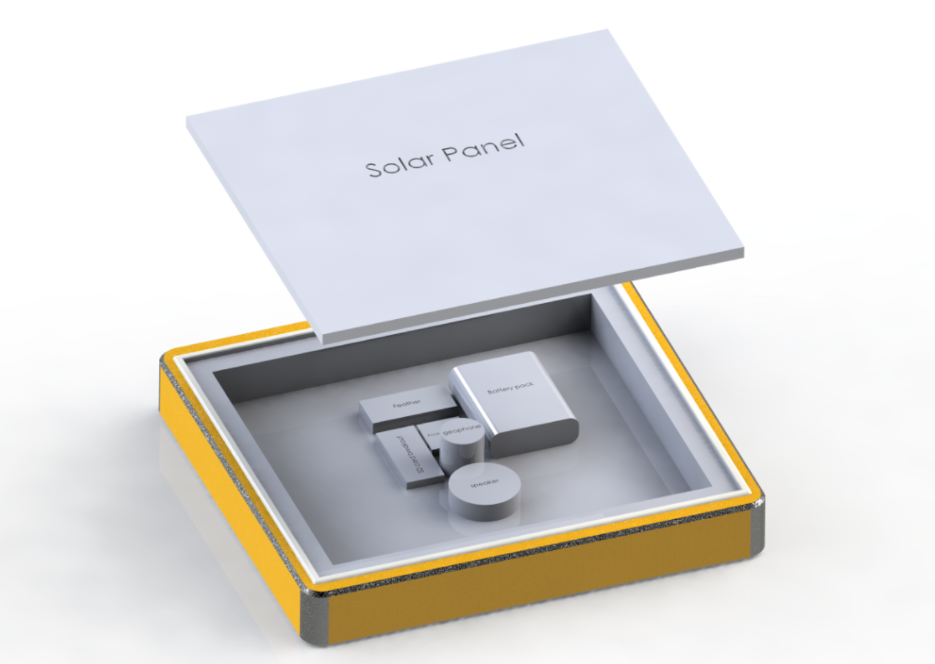
\includegraphics[width=0.6\textwidth]{alpha_enclosure}
\caption{}
\label{fig:alpha_enclosure}
\end{figure}


\subsection{Intermediate Prototypes}


Now that we were extracting data from the accelerometer and bringing into the feather, we then needed to feed this information to some where to sort the the data and make this into a meaningful.  
	
    The Azure platform is what we decided to go with in the database, with it a vast amount of tools and things to help us get started. We quickly learned that we knew very little about databases, and only understood them at a very basic functional level. After researching for a while make a few bumps along the way we finally got data to transmit. The next part involved integrating the geophone and creating database side functions that, relayed triggers, stored the data, and graphed the data for analysis.  
	
    Here we reached our system leveled design (SLD) in Figure \ref{fig:SLD} (see Appendix II) which included most parts of the project and their functions in the system. The SLD made up our final BOM (see Appendix I).
	
    from our second more refined version the the enclosure we very quickly that our material was limited and that our initial design required a lot more material than we had access to, but we knew that the parts would fit inside it, secure and properly mounted to the enclosure, we just needed to test the spacing 
\begin{figure}[H]
\centering
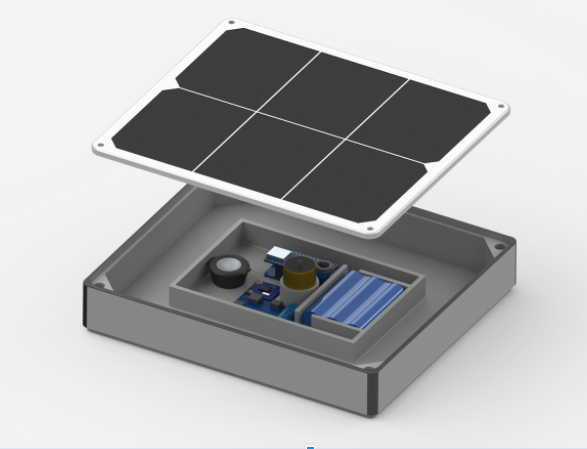
\includegraphics[width=0.6\textwidth]{beta_enclosure}
\caption{}
\label{fig:beta_enclosure}
\end{figure}
\subsection{Final Prototype}


After struggling with azure and trying to get the database working we were able to get data at a steady stream for a decent amount of time and were able to graph this data locally. Issues that remain exist in the database, still working on stream analytics, the ability to set triggers and sound the speaker that exists on the prototype. We plan to further improve this functionality, and refine data points gathered from the sensor. 
	For the enclosure we completely revamped the design, making it more modular. we added mounting points so that the box could be mounted to the wall we made the final prototype out of nylon because we found the PLA to be brittle and more susceptible to shock and impact. We also added a sheet of acrylic to secure that enclosure more firmly to the solar panel.  
\begin{figure}[H]
\centering
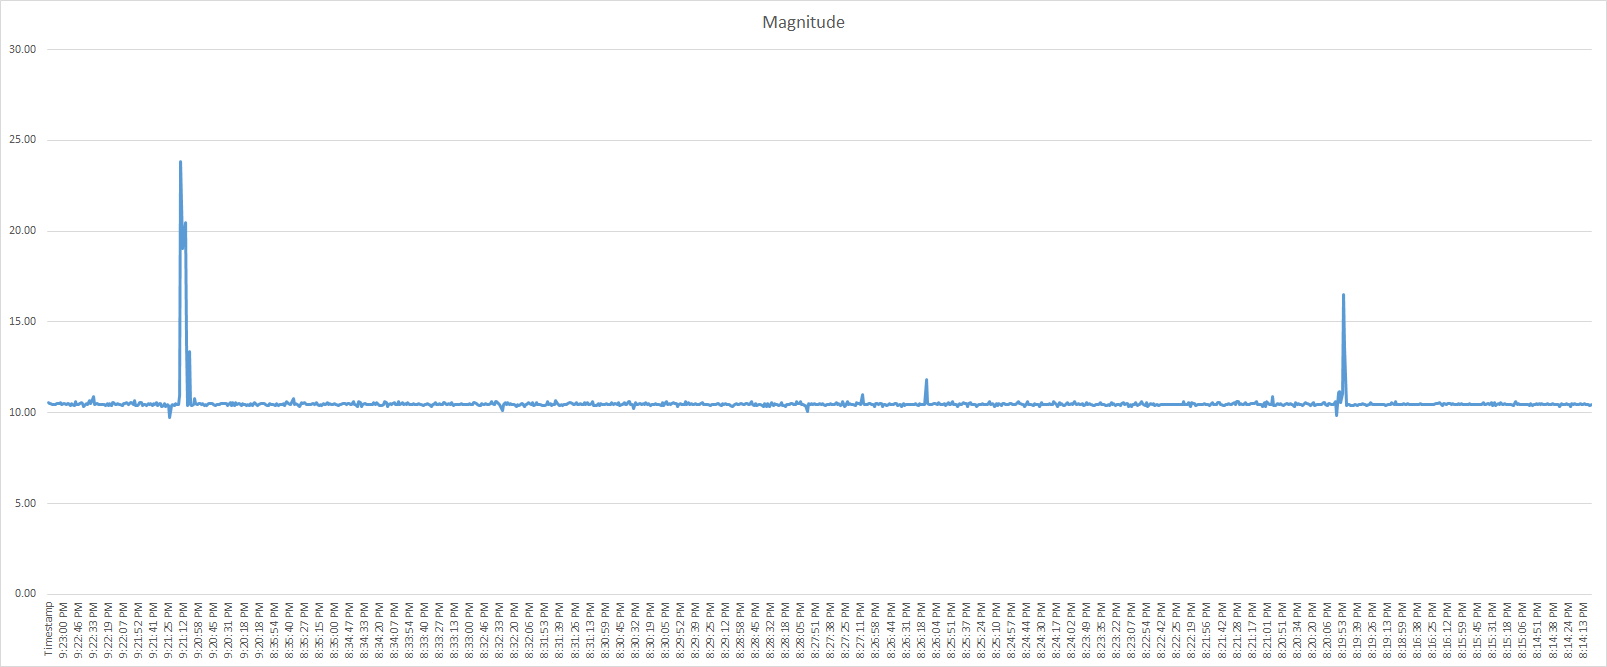
\includegraphics[width=1\textwidth]{grdata_azure}
\caption{Graph of data pulled via PowerBI from azure}
\label{fig:graphical data}
\end{figure}

\begin{figure}[H]
\centering
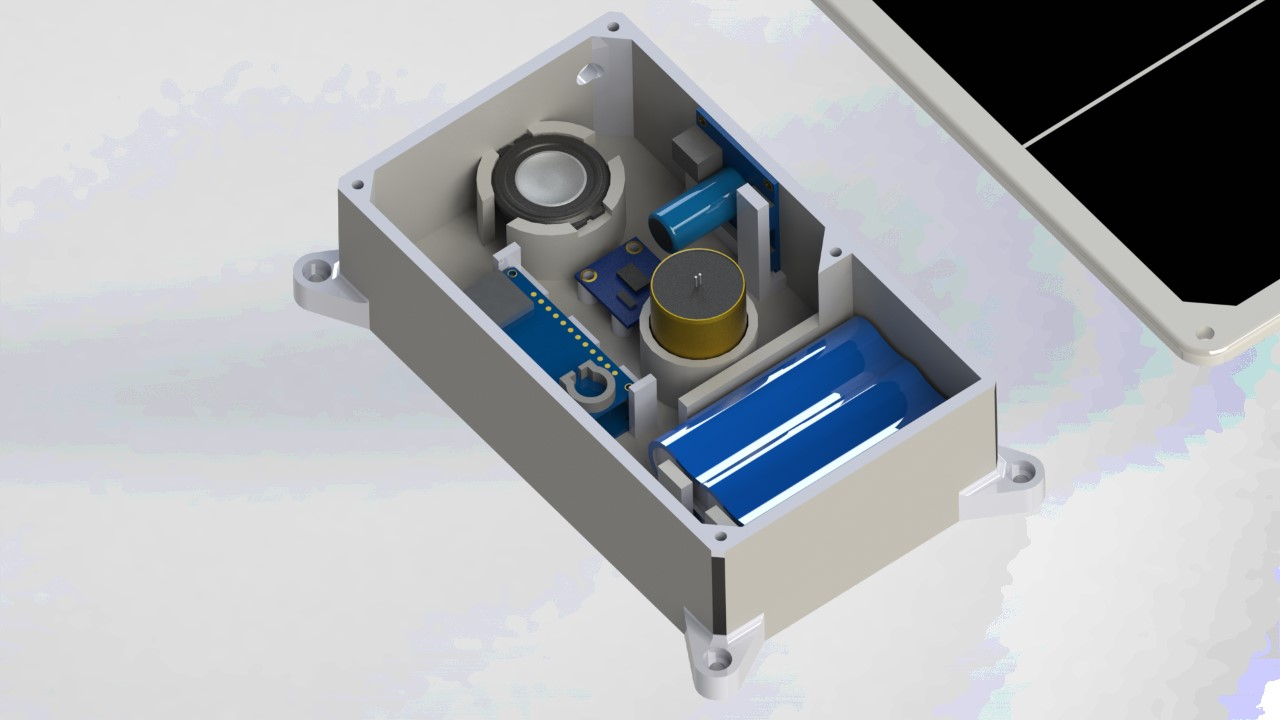
\includegraphics[width=0.6\textwidth]{final_assembly}
\caption{Final Solidworks drawing }
\label{fig:final_sldrprt}
\end{figure}

\begin{figure}[H]
\centering
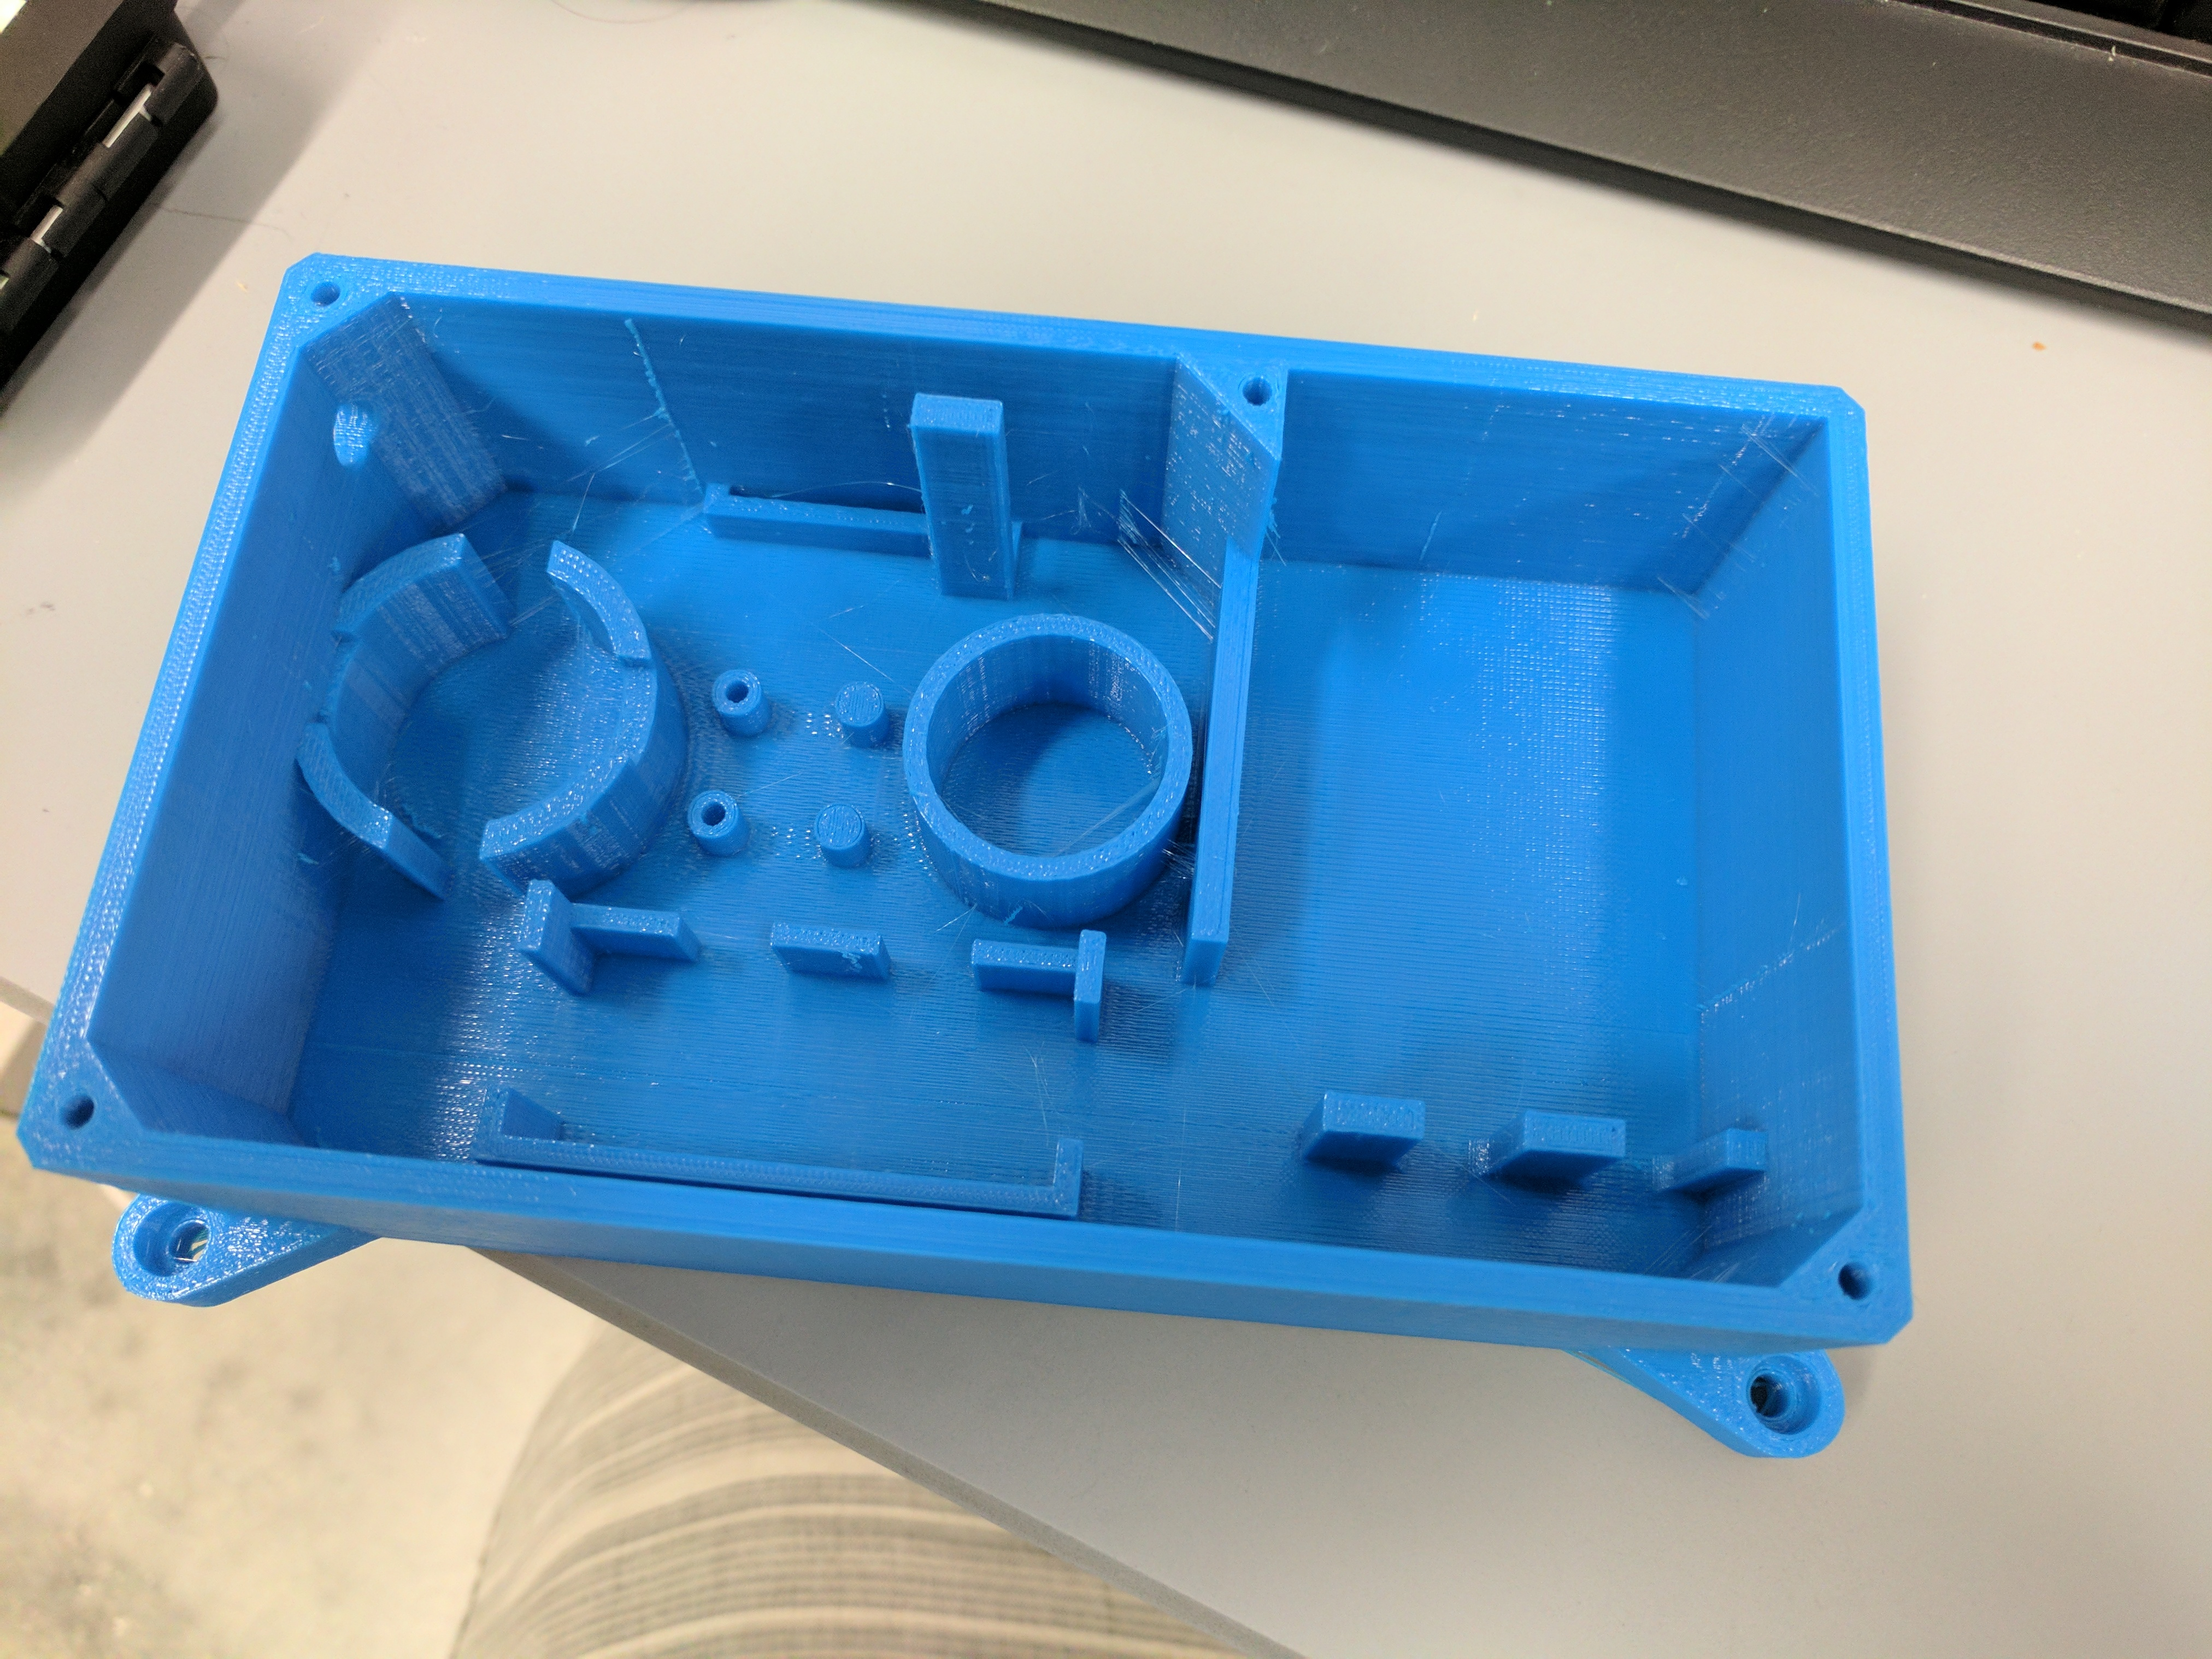
\includegraphics[width=0.6\textwidth]{enclosure}
\caption{Printed Enclosure out of PLA}
\label{fig:enclosure}
\end{figure}

%% Section
\section{Related Design Activities}

This was a very interesting project to work on. Not only was it helpful in developing the teams project management skills, it also helped us develop our critical thinking skills. We were not just given parts and told to make them work, or communicate with each other. We were given a prompt, and given a blank check to figure out a solution. This allowed us to be really creative, and increase our knowledge and skillset. While at the same time, it put pressure on us to do our research to avoid moving in the wrong direction.

\subsection{Risk Examination}

{When initially starting the project, the first thing we had to do was familiarize ourselves with what constitures a vibration sensor. How they work, what goes into making them, and how they are used. Then we had to create a list of parts we would be purchasing to build the sensor, we had to research all the parts individually to make sure there would be no conflict. To avoid being setback in case some of the parts were faulty or dead on arrrival, we ordered multiple of the more important parts. } 

\subsection{Skills Acquired During This Project}
{We were fortunate enough to learn plenty from actually implementing the project. We had to experiment and work with multiple software, to make both the virtual and hardware portions of the project. The first portion of the project we implemented was the hardware. The main piece in the hardware was the Arduino Feather M0 microcontroller. All the other pieces of the sensor are connected to and by the arduino feather. To program the feather, and all the other sensor components, we used the Arduino IDE(Integrated Development Environment). For the cloud implementation of the sensor, we had to familiarize ourselves with a couple of different solutions to find the one that worked best for us. We initially wanted to use a NOSql(Non Structured Query Language) solution known as MongoDB. NoSql is a storage method similar to SQL, except that it does not store the data into tables. Rather, all pieces of information are given an ID, then data belonging to the ID are given a reference object by which they can be filtered similar to columns.  Then, we figured out how to use Microsoft Azure to implement all of our cloud storage needs. We just needed to learn how to use the Azure web interface, query commands for the storage, and the cloud to device messaging functionality.}

%% Section
\section{Conclusions and Future Work}


After being chosen for this project at the beginning of the fall semester of 2016, we have completed a significant amount of work we have a working sensor, albeit not to the standard we initially set for ourselves. The main sensor works well, but the important cloud connectivity remains elusive to us. There are certain parts of the project that could have been implemented better, and others that are closed to being done but still unfinished.


\subsection{Conclusions and Project Summary}
While we were not able to reach 100\% percent completion, we have managed to reach a level of completion surpassing 80\%. The main goals of the project were to design a sensor that could connect to the internet and transfer data remotely, be able to last close to 4 weeks on a single charge, and portability. We were able to design a small, compact sensor that is easily transportable form site to site. It can be laid on the floor, or mounted to a surface useing the mounting holes on the edge of the enclosure. To account for the battery being drained from continuous use by the components, we implemented a solar panel to charge the battery. The solar panel also helps reduce the load on the battery. As for the cloud connectivity, we were able to get the sensor system to send the data to Azure storage, and were able to monitor the sensor's activity remotely. Unfortunately, we are unable to conduct further testing due to lack of funding.  

If we were in possession of a sufficient amount of funds to finish the Microsoft Azure implementation, we would have been able to finish the cloud connectivity aspect of the sensor. We figured out how to pull the data from the storage, and extract what we needed. This would be done with Microsoft Power BI. Then we would perform an FFT (Fast Fourier Transform) to pull the frequency from the sensor data, and resend that new value to the cloud which would then decide if an alert should be sent to the sensor or not.

 

\subsection{Future Work}

Although we managed to do a lot of the work and implementation necessary , we did not manage to fully complete the sensor. We were able to achieve connection to Azure cloud storage and transmit messages and data, we were unable to further test it due to lack of funds. Issues that remain exist in the database, still working on stream analytics, the ability to set triggers and sound the speaker that exists on the prototype. We plan to further improve this functionality, and refine data points gathered from the sensor. In terms of improvements we could have made, we could have used a larger budget, or not bought secondaries for certain parts. 

\newpage
\appendix 

\section{Appendix I}

\begin{center}
\textbf{Bill of Materials}\\ Smart Vibes
\end{center}
\begin{table}[H]
	\centering
	\resizebox{\columnwidth}{!}{%
	\begin{tabular}{l|l|c|l|l|r|c|c}
    	Vendor ID & Part Number & Quantity & Price/Unit & Part Description & Cost & Vendor & Datasheet\\ \hline
    	1120 & LSM303 & 2 & \$14.95 & Accelerometer & \$29.90 & \href{https://www.adafruit.com/products/1120}{Adafruit} & \href{https://cdn-shop.adafruit.com/datasheets/LSM303DLHC.PDF}{PDF} \\
    	2693 & N.A. & 2 & \$19.95 & 16GB MicroSD Card & \$39.90 & \href{https://www.adafruit.com/products/2693}{Adafruit} & \href{https://www.adafruit.com/products/2693}{Website} \\
    	2922 & N.A. & 2 & \$8.95 & SD Card Breakout & \$17.90 & \href{https://www.adafruit.com/products/2922}{Adafruit} & \href{http://www.nxp.com/documents/data_sheet/PCF8523.pdf}{PDF} \\
    	& & & & with Coin Cell Battery & & & \\
    	%380 & CR1220 & 2 & \$0.95 & Coin Cell Battery & \$1.90 & \href{https://www.adafruit.com/products/380}{Adafruit} & \href{https://www.adafruit.com/products/380}{Website} \\
    	3061 & N.A. & 1 & \$34.95 & Adafruit Feather & \$34.95 & \href{https://www.adafruit.com/products/3061}{Adafruit} & \href{https://learn.adafruit.com/system/assets/assets/000/030/130/original/atmel-42181-sam-d21_datasheet.pdf?1453847579}{PDF} \\
    	353 & N.A. & 2 & \$29.50 & 6600 mAh 3.7V Lithium- & \$59.00 & \href{https://www.adafruit.com/product/353}{Adafruit} & \href{https://cdn-shop.adafruit.com/product-files/353/C450_-_ICR18650_6600mAh_3.7V_20140729.pdf}{PDF} \\
    	& & & & Ion Battery & & \\
    	2747 & N.A. & 1 & \$88.95 & Solar Panel & \$88.95 & \href{https://www.adafruit.com/products/2747}{Adafruit} & \href{https://www.voltaicsystems.com/9-watt-panel}{Website} \\
    	579-MCP73871-2CCI/ML & MCP73871-2CCI/ML & 1 & \$1.94 & Battery Charger & \$1.94 & \href{http://www.mouser.com/ProductDetail/Microchip-Technology/MCP73871-2CCI-ML/?qs=qXsUupcbpXyQfJ2clznZxw\%3D\%3D}{Mouser} & \href{http://www.mouser.com/ds/2/268/22090a-52174.pdf}{PDF} \\
		N.A. & 474-SEN-11744 & 1 & \$61.25 & Geophone & \$61.25 & \href{http://www.mouser.com/ProductDetail/SparkFun-Electronics/SEN-11744/?qs=\%2fha2pyFaduhLW6YoPw5UUIdTRP1X\%252btPruyfOHvl8\%2fY0\%3d}{Mouser} & \href{http://cdn.sparkfun.com/datasheets/Sensors/Accelerometers/SM-24\%20Brochure.pdf}{PDF} \\
    	 39RL33 & N.A. & 1 & \$34.75 & White Nylon Filament & \$34.75 & \href{https://www.grainger.com/product/FILABOT-White-Filament-39RL33}{Grainger} & \href{https://www.grainger.com/product/FILABOT-White-Filament-39RL33}{Website} \\
    	 & & & & for 3-D Printer & & \\
    	 2788 & N.A. & 1 & \$0.95 & DC Jack Adapter Cable & \$0.95 & \href{https://www.adafruit.com/products/2788}{Adafruit} & \href{https://www.adafruit.com/products/2788}{Website} \\
    	 & & & & for Battery Charger & & & \\
    	 581-TAP475K016SCS & TAP475K016SCS & 1 & \$0.67 & Tantalum Capacitor & \$0.67 & \href{http://www.mouser.com/ProductDetail/AVX/TAP475K016SCS/?qs=sGAEpiMZZMtZ1n0r9vR22d\%252b8XmbM9QM8L4TTXY3LGQ8\%3d}{Mouser} & \href{http://www.mouser.com/ds/2/40/tap-776819.pdf}{PDF} \\
    	 & & & & for Battery Charger & & & \\
    	 261 & N.A. & 1 & \$0.75 & JST 2-pin Cable & \$0.75 & \href{https://www.adafruit.com/product/261}{Adafruit} & \href{https://www.adafruit.com/product/261}{Website} \\
    	 & & & & for Battery Charger & & & \\
    	 	PMT-37N28AL01-04-ND & PMT-37N28AL01-04 & 1 & \$8.57 & Speaker & \$8.57 & \href{http://www.digikey.com/product-detail/en/peerless-by-tymphany/PMT-37N28AL01-04/PMT-37N28AL01-04-ND/6211115}{Digi-Key} & \href{http://www.tymphany.com/wp-content/themes/pathfinders/cache/pdfs/PMT-37N28AL01-04.pdf}{PDF} \\
        2308 & N.A. & 1 & \$2.50 & Antenna with uFL & \$2.50 & \href{https://www.adafruit.com/products/2308}{Adafruit} & \href{https://www.adafruit.com/products/2308}{Website} \\
    	 & & & & Connector & & & \\ \hline
    	Total Cost & & & & & \$381.98 &
	\end{tabular}%
	}
    %\caption{Bill of materials.}
    \label{tab:bom}
\end{table}

\pagebreak

\section{Appendix II}
\begin{figure}[h]
\centering
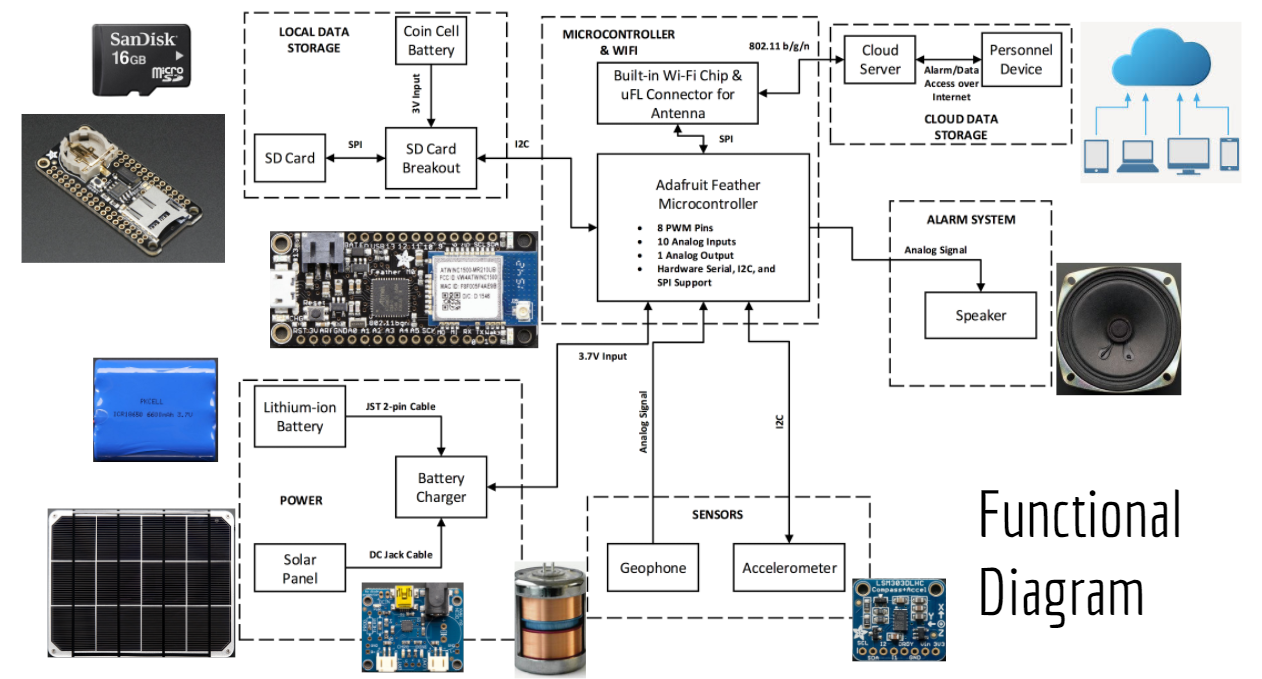
\includegraphics[width=0.9\textwidth]{Functional_diagram_p2}
\caption{Function diagram }
\label{fig:SLD}
\end{figure}

\end{document}				
